\section{Поверхности}

Чтобы увидеть особенности контактов между биомолекулами, полезно построить их поверхности. Поверхности можно описывать на основе различных физико-химических свойств молекулы, наиболее распространенные способы: поверхность доступности и вытеснения растворителя (SAS, SES), Ван~дер~Ваальсова поверхность (VdW) и различные поверхности электронной плотности (EDS).
\begin{figure}[h!]
  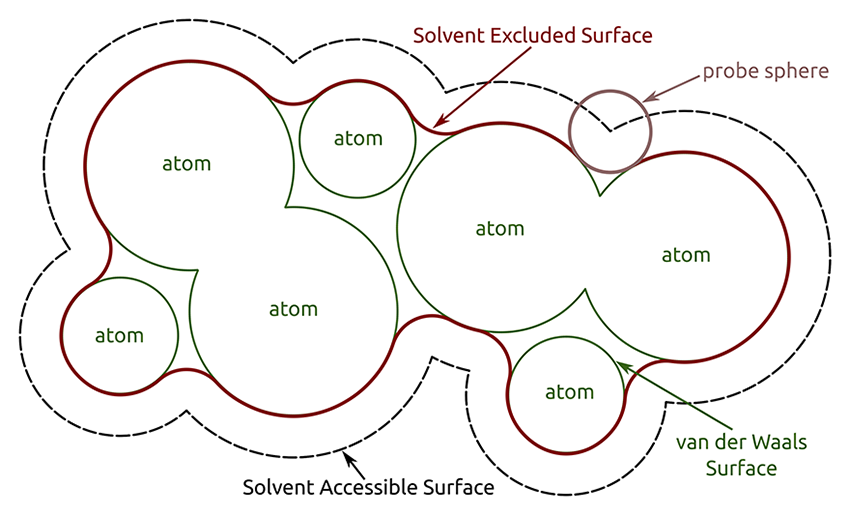
\includegraphics[width=\linewidth]{Figures/Surface.png}
  \caption{\textit{Способы построения поверхностей в UCSF Chimera.}}
  \label{fig:surf}
\end{figure}\clearpage

\subsection*{Задание~7}
\begin{enumerate}
    \item Постройте для каждого белка поверхность вытеснения растворителя \textit{(см. задание~3.\ref{task:surf})}.
    
    \item В окне Model Panel скройте лишние модели, оставив один белок и его поверхность.
    
    \item Откройте диалог\quad\texttt{Tools~> De\-pic\-tion~> Per-Mo\-del Clip\-ping}.
    
    \item Выберите модель <<MSMS main surface \dots>> и поставьте чекбокс\quad\texttt{En\-able clip\-ping}.
    
    \item Настройте положение секущей плоскости, поставив чекбокс в поле\\
    \texttt{Adjust clipping with mouse as below}.
    
    \item В диалоговом окне\quad\texttt{Sur\-face cap\-ping}\quad настройте свойства секущей плоскости.
\end{enumerate}